\documentclass[12pt]{article}
\usepackage[ansinew]{inputenc} % ASCII (Western CP)
\usepackage{graphicx}
\usepackage{color}
\usepackage[colorlinks]{hyperref}
\usepackage{geometry}
\usepackage{amsmath}
\usepackage{tabularx}
\usepackage{multirow}
\usepackage{subfigure}
\usepackage{float}

\geometry{left=2.5cm,right=2.5cm,top=2.5cm,bottom=2.5cm}

\title{Machine Learning - HW1 \& 2}
\author{Pang Liang\\ Student No. 201418013229033}

\begin{document}
\maketitle

%    \begin{table}[!hbp]
%      \centering
%      \begin{tabular}{|c|c||c|c|}
%        \hline
%        $x_1$ & $x_2$ & $p(c=0|x_1, x_2)$ & $p(c=1|x_1, x_2)$ \\
%        \hline
%       0 & 0 & 0.25 & 0.75 \\
%       \hline
%        0 & 1 & 0.25 & 0.75 \\
%        \hline
%        1 & 0 & 1. & 0. \\
%        \hline
%        1 & 1 & 0.6 & 0.4 \\
%        \hline
%      \end{tabular}

%      \caption{Values of $p(y | x_1, x_2)$.} \label{table1}
%    \end{table}

\section{Problem1 - Bayes Classifier}

%    \begin{table}[!hbp]
%      \centering
%      \begin{tabular}{|c|c|c||c|}
%        \hline
%        $x_1$ & $x_2$ & $y$ & $p(y, x_1, x_2)$ \\
%        \hline
%        0 & 0 & 0 & 0.0625 \\
%        \hline
%        0 & 0 & 1 & 0.1875 \\
%        \hline
%        0 & 1 & 0 & 0.0625 \\
%        \hline
%        0 & 1 & 1 & 0.1875 \\
%        \hline
%        1 & 0 & 0 & 0.1875 \\
%        \hline
%        1 & 0 & 1 & 0.0 \\
%        \hline
%        1 & 1 & 0 & 0.1875 \\
%        \hline
%        1 & 1 & 1 & 0.125 \\
%        \hline
%      \end{tabular}

%      \caption{Values of $p(y , x_1, x_2)$.} \label{table1}
%    \end{table}

\begin{enumerate}
    \item Joint Bayes Classifier
    The joint distribution over all feature is that
    \begin{equation}
    p(y|x_1, x_2) =  \frac{p(x_1,x_2|y)*p(y)}{\sum_y p(x_1, x_2|y) p(y)}
    \end{equation}
    So we need estimate these probabilities given the train data. The $p(y, x_1, x_2)$ shows in \ref{table1}.

    \begin{table}[!hbp]
      \centering
      \begin{tabular}{|c||c|c|c|c|}
        \hline
        $y$ & $p(x_1=0,x_2=0 | y)$ & $p(x_1=0,x_2=1 | y)$ & $p(x_1=1,x_2=0 | y)$ & $p(x_1=1,x_2=1 | y)$ \\
        \hline
        0 & 0.125 & 0.125 & 0.375 & 0.375\\
        \hline
        1 & 0.375 & 0.375 & 0.000 & 0.250\\
        \hline
      \end{tabular}

      \caption{Values of $p(x_1, x_2 | y)$.}\label{table2}
    \end{table}

    \begin{equation}
    p(y = 0) = 0.5 , p(y = 1) = 0.5
    \end{equation}

    Then we predict the test data below:
    \begin{equation}
        \begin{split}
            p(y = 1|x_1 = 0, x_2 = 1) &= 0.75
        \end{split}
    \end{equation}

    \begin{equation}
        \begin{split}
            p(y = 1|x_1 = 1, x_2 = 0) &=  0
        \end{split}
    \end{equation}

    \begin{equation}
        \begin{split}
            p(y = 0|x_1 = 1, x_2 = 1) &= 0.6
        \end{split}
    \end{equation}


    \item Naive Bayes Classifier
    For Naive Bayes we assume that $p(x_1, x_2 | y) = p(x_1 | y) * p(x_2 | y)$. So
    \begin{equation}
    p(y|x_1, x_2) =  \frac{p(x_1|y)*p(x_2|y)*p(y)}{\sum_y p(x_1|y)*p(x_2|y)*p(y)}
    \end{equation}

    Then we only need $p(x_1 | y)$ and $p(x_2 | y)$ below:

    \begin{table}[!hbp]
      \centering
      \begin{tabular}{|c||c|c|}
        \hline
        $y$ & $p(x_1=0 | y)$ & $p(x_1=1 | y)$  \\
        \hline
        0 & 0.25 & 0.75 \\
        \hline
        1 & 0.75 & 0.25 \\
        \hline
      \end{tabular}

      \caption{Values of $p(x_1 | y)$.}\label{table2}
    \end{table}

    \begin{table}[!hbp]
      \centering
      \begin{tabular}{|c||c|c|}
        \hline
        $y$ & $p(x_2=0 | y)$ & $p(x_2=1 | y)$  \\
        \hline
        0 & 0.5 & 0.5 \\
        \hline
        1 & 0.375 & 0.625 \\
        \hline
      \end{tabular}

      \caption{Values of $p(x_2 | y)$.}\label{table3}
    \end{table}

    \begin{equation}
    p(y = 0) = 0.5 , p(y = 1) = 0.5
    \end{equation}

    Then we predict the test data below:
    \begin{equation}
        \begin{split}
            p(y = 1|x_1 = 0, x_2 = 1) &= \frac{0.75*0.625}{0.75*0.625+0.25*0.5}\\
            &= 0.789
        \end{split}
    \end{equation}

    \begin{equation}
        \begin{split}
            p(y = 1|x_1 = 1, x_2 = 0) &= \frac{0.25*0.375}{0.25*0.375+0.75*0.5}\\
            &= 0.2
        \end{split}
    \end{equation}

    \begin{equation}
        \begin{split}
            p(y = 0|x_1 = 1, x_2 = 1) &=  \frac{0.75*0.5}{0.75*0.5+0.25*0.625}\\
            &= 0.706
        \end{split}
    \end{equation}


\end{enumerate}


\section{Problem2 - Gaussian Bayes Classifiers}
See Code \href{./CodeAndData#1/H1P2.m}{\textbf{H1P2.m}} .
\begin{enumerate}
    \item Plot the iris data X in 2-D space

    \begin{figure}[H]
      \centering
      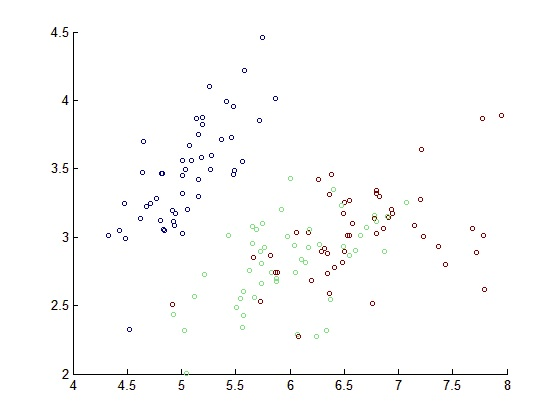
\includegraphics[width=8cm]{fig/2-0.jpg}\\
      \caption{Data distribution}\label{fig1}
    \end{figure}

    \item Plot each of Gaussian Kernels on top of the data

    \begin{figure}[H]
      \centering
      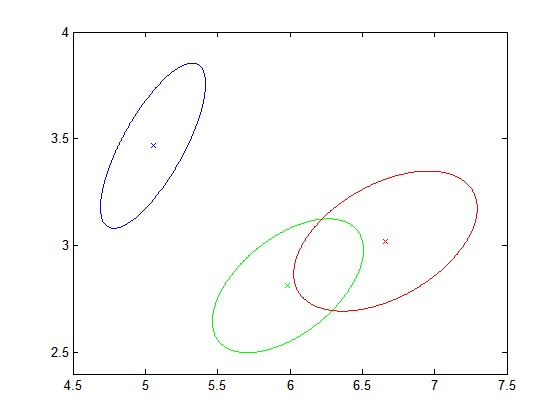
\includegraphics[width=8cm]{fig/2-1.jpg}\\
      \caption{Estimated Gaussian Kernels}\label{fig1}
    \end{figure}

    \item Using Gaussian Bayes Classify (with free covariances)

    \begin{figure}[H]
      \centering
      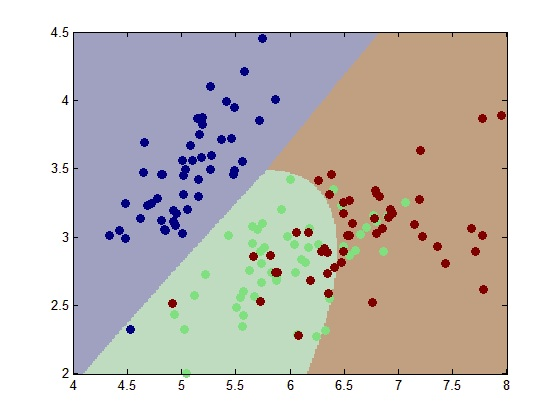
\includegraphics[width=8cm]{fig/2-2.jpg}\\
      \caption{Class Boundary}\label{fig1}
    \end{figure}
    The shape of the boundary are the parts of a ellipse/circle.

    \item Using Gaussian Bayes Classify (with equal covariances)

    \begin{figure}[H]
      \centering
      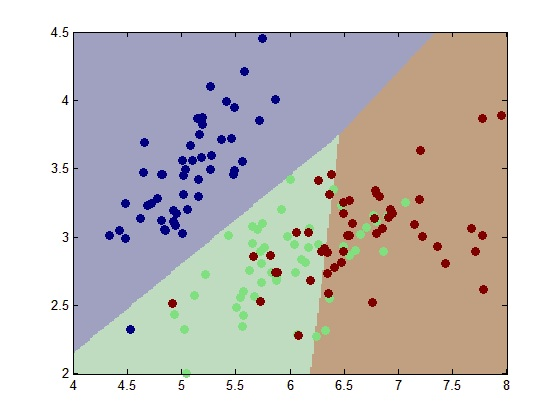
\includegraphics[width=8cm]{fig/2-3.jpg}\\
      \caption{Class Boundary}\label{fig1}
    \end{figure}
    The shape of the boundary are the straight lines.

    \item Poly Classify ($p = 2,3,4$)

    \begin{figure}[H]
        \centering
        \subfigure[$p=2$]{
            \label{Fig.sub.1}
            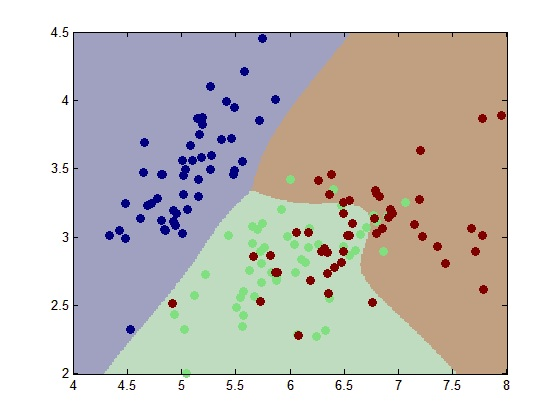
\includegraphics[width=0.3\textwidth]{fig/2-4-2.jpg}}
        \subfigure[$p=3$]{
            \label{Fig.sub.2}
            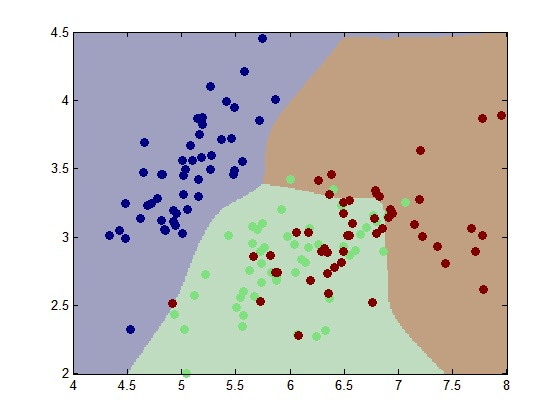
\includegraphics[width=0.3\textwidth]{fig/2-4-3.jpg}}
        \subfigure[$p=4$]{
            \label{Fig.sub.3}
            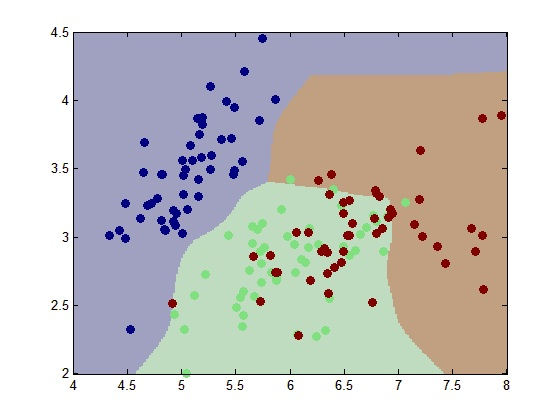
\includegraphics[width=0.3\textwidth]{fig/2-4-4.jpg}}
        \caption{Different Poly Level, Draw Class Boundary}
        \label{Fig.lable}
    \end{figure}

    With the increasing of $p$, the boundary of each classes become more complex. And it's become easier to overfit on training set.

\end{enumerate}


\section{Problem3 - SVM}
See Code \href{./H1P3.m}{\textbf{H1P3.m}} .
\begin{enumerate}
    \item The optimal hyperplane is $x_1+x_2-3=0$.
    And the margin is $\frac{\sqrt{2}}{2}$.
        \begin{figure}[H]
          \centering
          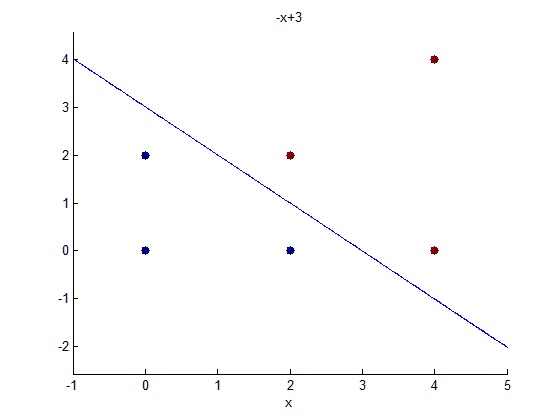
\includegraphics[width=8cm]{fig/3-1.jpg}\\
          \caption{Class Boundary}\label{fig1}
        \end{figure}
    \item The support vectors are: $(2,2)$,$(4,0)$,$(2,0)$,$(0,2)$. 

\end{enumerate}

\section{Problem4 - Run SVMs}
\begin{enumerate}
    \item
    See Code \href{./H1P4.m}{\textbf{H1P4.m}} .
    \item
    Use linear SVM get Accuracy of $89.3\%$. \\
    Use default SVM get Accuracy of $92.4\%$. \\
    \begin{figure}[H]
       \centering
       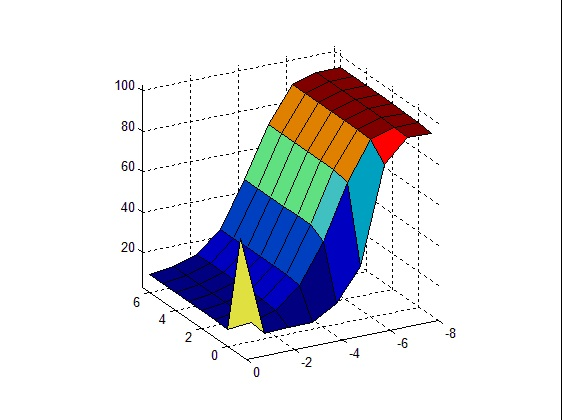
\includegraphics[width=10cm]{fig/svm.jpg}\\
       \caption{Grid Search.}\label{fig1}
    \end{figure}
    In my experiments, to set $C=2^3=8$ and $gamma=2^{-7}$ is the best parameter. Cross Validation accuracy is $94.45\%$, and Test accuracy is $95\%$.

\end{enumerate}

\end{document}
